% !TeX program = xelatex*2
% !TeX root = ../elegantnote.tex
\section{函数逼近}
\subsection{最佳一致逼近}
\begin{definition}
    设$f\in C[a,b],p_{n}\in H_{n}=\mathrm{Span}\{1,x,\cdots,x^{n}\},$称
    \[
        \Delta(f,p_n)=\parallel f-p_n\parallel_\infty=\max_{a\leq x\leq b}\mid f(x)-p_n(x)\mid 
    \]
    为$p_{n}$与$f$的偏差
    \[
        E_{n}=\operatorname*{inf}_{p_{n}\in H_{n}}\Delta(f,p_{n})
    \]
    为$p_{n}$与$f$的最小偏差
    
    若$\exists p_{n}^{*}\in H_{n},$使$\Delta(f,p_{n}^{*})=E_{n}$,则称$p^{*}$为$f$在$\left[ a,b \right]$上的最佳一致逼近多项式,简称最佳逼近多项式。
\end{definition}
\begin{definition}[偏差点]
    设$f\in C[a,b],p_{n}\in H_{n}$,若$\exists x_0\in[a,b]$使得
    \[
        \mid f(x_0)-p(x_0)\mid=\Delta(f,p)=\mu 
    \]
    则称$x_0$是$p$关于$f$的偏差点。

    \begin{itemize}
        \item 若$p(x_{0})-f(x_{0})=\mu,$则称$x_0$为正偏差点。
        \item 若$p(x_{0})-f(x_{0})=-\mu,$则称$x_0$为负偏差点。
    \end{itemize}
\end{definition}
\begin{theorem}
    设$p_{n}^{*}\in H_{n}$为$f\in\left[ a,b \right]$的最佳一致逼近多项式,则$p_{n}^{*}$关于$f$的正负偏差点同时存在。
\end{theorem}
\subsubsection{Chebyshev多项式}
\begin{definition}[Chebyshev多项式]
    当权函数$\rho(x) = \dfrac{1}{\sqrt{1-x^2}}$,区间为$\left[ -1,1 \right]$时,得到的正交多项式就是Chebyshev多项式,它可以表示为
    \[
        T_{n}(x) = \cos\left( n\arccos x \right),\quad |x|\leqslant 1
    \]
\end{definition}
\begin{corollary}
    递推关系
    \[
        \begin{array}{c}
            T_0(x) = 1,\quad T_{1}(x) = x\\
            T_{n+1}(x) = 2xT_{n}(x)-T_{n-1}(x),\quad (n = 1,2,\cdots,n)
        \end{array}
    \]
    由递推关系式还可以得到$T_{n}(x)$的最高项系数为$2^{n-1}(n\geqslant 1)$
\end{corollary}
\begin{proof}
    由和差化积$\cos(n+1)x-\cos(n-1)x = 2\cos(nx)\cos(x)$并令$x = \arccos x$得到
    \[
        \begin{array}{c}
            T_{n+1}(x)-T_{n-1}(x) = 2xT_{n}(x)\\
            \Rightarrow T_{n+1}(x) = 2xT_{n}(x) + T_{n-1}(x)
        \end{array}
    \]
    证毕!
\end{proof}
\begin{corollary}
    $T_{n}(x)$对零的偏差最小,可以写成如下定理。
\end{corollary}
\begin{theorem}\label{theo:Tx-0min}
    在区间$[-1,1]$上所有最高项系数为1的一切$n$次多项式中,$\widetilde{T}_{n}(x) = \dfrac{1}{2^{n-1}}T_{n}(x)$与零的偏差最小,其偏差为$\dfrac{1}{2^{n-1}}$\Stars{5}{}
\end{theorem}
\begin{note}
    $T_{n}(x)$的函数及其图形如下:
    \begin{figure}[H]
        \centering
        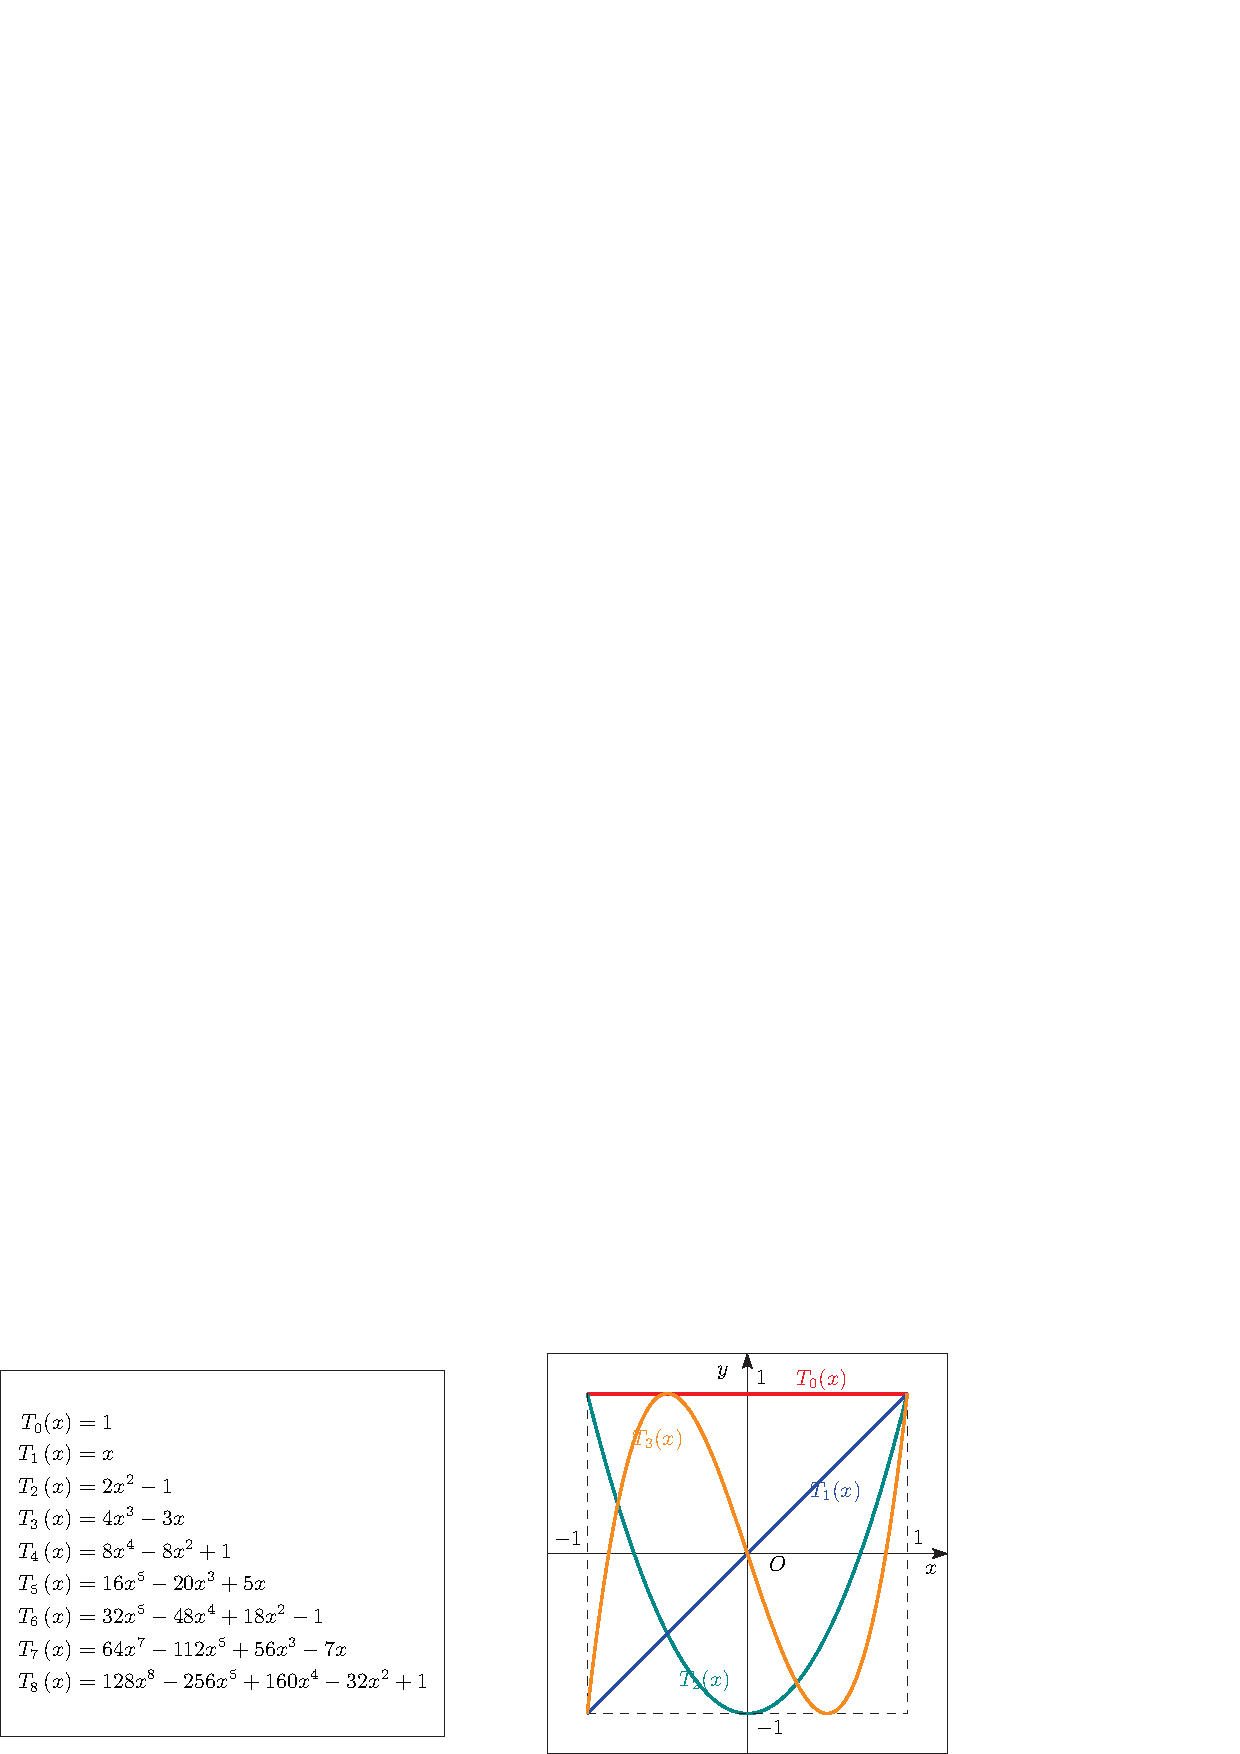
\includegraphics[width = .86\textwidth]{image/ChebyshevTx.pdf}
    \end{figure}
\end{note}
\begin{note}
    性质:
    \begin{enumerate}
        \item 正交性
        \[
            (T_n,T_m)=\begin{cases}
                0&m\neq n\\
                \dfrac{\pi}{2}& m=n\neq 0\\
                \pi & m=n=0
            \end{cases}
        \]
        \item 递推关系$T_{n+1}(x) = 2xT_{n}(x) + T_{n-1}(x)$
        \item 奇偶性$T_n(-x)=(-1)^nT_n(x)$
    \end{enumerate}
\end{note}
\begin{example}
    设$f(x) = x^4$,在$[-1,1]$上求$H_3$中的最佳逼近多项式。\Stars{3.5}{}

    \begin{solution}
        由定理~\ref{theo:Tx-0min}知道
        \[
            \dfrac{f(x)-p_{3}^{*}(x)}{1} = \dfrac{T_{4}(x)}{2^{4-1}}    
        \]
        其中$T_{4}\left(x\right) =8x^4-8x^2+1$,故而
        \[
            \begin{array}{ll}
                p_{3}^{*}(x) &= f(x)- \dfrac{T_{4}\left(x\right)}{2^{3}}\\
                &=x^2-\dfrac{1}{8}
            \end{array}
        \]
    \end{solution}
\end{example}
\begin{example}
    求$f(x) = 2x^3+x^2+2x-1$在$[-1,1]$上的最佳一致逼近多项式。\Stars{4}

    \begin{solution}
        \[
            \colorbox{red!30}{$\dfrac{f(x)-p_{2}^{*}(x)}{a_n}$} = \dfrac{T_{3}(x)}{2^{n-1}}\colorbox{red!30}{变成最高次系数为1的多项式}
        \]
        故
        \[
            p_{2}^{*}(x) = f(x)-\dfrac{1}{2}T_{3}(x) = x^2+\frac{7}{2}x-1
        \]
    \end{solution}
\end{example}
\begin{theorem}
    若$P(x)\in H_{n}$是$f(x)\in C[a,b]$的最佳逼近多项式,则$P(x)$同时存在正负偏差点。
\end{theorem}
\begin{theorem}[Chebyshev]\label{theo:Chebyshev}
    $p_n^*\in H_n$是$f\in C\left[ a,b \right]$的最佳逼近多项式的充要条件是:在$\left[ a,b \right]$上至少有$n+2$个轮流为正负的偏差点,即至少有$n+2$个点$a\leqslant x_1\leqslant x_2\leqslant \cdots\leqslant x_{n+2}\leqslant b$使得
    \[
        p_{n}^{*}(x_k)-f(x_k) = (-1)^{k}\sigma\| f-p_{n}^* \|_{\infty},\,\sigma = \pm 1,\,k =1,2,\cdots,n+2 
    \]
    上述点$\left\{ x_k \right\}_{1}^{n+2}$称为切比雪夫交错点。
\end{theorem}
\begin{corollary}
    设$f\in C[a,b]$,则在$H_n$中的最佳逼近多项式是唯一的。
\end{corollary}
\begin{corollary}
    若$f\in C[a,b]$,则其最佳逼近多项式$p_{n}^{*}(x)\in H_n$是$f$的一个拉格朗日多项式。
\end{corollary}
\begin{example}
    假定$f(x)\in C^{2}[a,b]$,且$f^{\prime\prime}(x)$在$(a,b)$内不变号,求最佳一次逼近多项式$P_1(x) = a_0+a_1x$。\Stars{5}{}
    \begin{solution}
        根据定理~\ref{theo:Chebyshev}可知,至少有3个点$a\leqslant x_1\leqslant x_2\leqslant x_3\leqslant b$使得
        \[
            P_{1}(x_k)-f(x_k) = (-1)^{k}\sigma\max\limits_{a\leqslant x\leqslant b}|P_{1}(x)-f(x)|
        \]
        由于$f^{\prime\prime}(x)$在$(a,b)$内不变号,故$f'(x)$单调,$f'(x)-a_1$在$(a,b)$内只有一个零点,记为$x_2$,于是
        \[
            P'_{1}(x_2)-f'(x_2) = a_1-f'(x_2) = 0,\quad\text{即}\,f'(x_2) = a_1
        \]
        \colorbox{red!50}{另外两个偏差点必在区间端点},即$x_0 = a,x_1  =b$,且满足
        \[
            P_{1}(a)-f(a) = P_{1}(b)-f(b) = -[P_{1}(x_2)-f(x_2)]
        \]
        由此得到
        \[
            \left\{
                \begin{array}{l}
                    a_0+a_1a-f(a)=a_0+a_1b-f(b)\\
                    a_0+a_1a-f(a)=f(x_2)-(a_0+a_1x_2).
                \end{array}
            \right.
        \]
        解得
        \[
            \begin{array}{l}
                a_1 = \dfrac{f(b)-f(a)}{b-a} = f'(x_2)\\
                a_0 = \dfrac{f(a)+f(x_2)}{2}-\dfrac{f(b)-f(a)}{b-a}\dfrac{a+x_2}{2}
            \end{array}
        \]
    \end{solution}
\end{example}
\begin{example}
    $f(x) = \sqrt{x^2+1}$,求$[0,1]$上的最佳一次逼近多项式。\Stars{2.5}
    
    \begin{solution}
        先求$x_2$和$f(x_2)$
        \[
            \begin{array}{l}
                f'(x_2) = \dfrac{x_2}{\sqrt{x_2^2+1}} = \dfrac{f(1)-f(0)}{1-0} = \sqrt{2}-1\approx 0.414\\
                \Rightarrow x_2  = \sqrt{\dfrac{\sqrt{2}-1}{2}}\approx 0.4551,\,f(x_2) = \sqrt{1+x_2^2} = 1.0986
            \end{array}
        \]
    \end{solution}
\end{example}
\subsection{最佳平方逼近}
\begin{definition}[正交函数]
    若$f(x),g(x)\in C[a,b]$满足
    \[
        (f,g) = \int_{a}^{b}\rho(x)f(x)g(x)\mathrm{d} x = 0,
    \]
    则称$f$与$g$在$[a,b]$上带权$\rho(x)$正交。若函数族$
    \varphi_{0}(x),\cdots,\varphi_{n}(x)$满足关系
    \[
        (\varphi_j,\varphi_k)=\int_a^b\rho(x)\varphi_j(x)\varphi_k(x)\mathrm{d}x=
        \left\{
            \begin{array}{ll}
                0, & j\neq k,\\
                A_k>0, & j=k,
            \end{array}
        \right.
    \]
    则称${\varphi_k}$是$[a,b]$上带权$\rho(x)$得正交族函数。
\end{definition}
\begin{theorem}
    若$(f,g)\in C[a,b]$,则有
    \[
        \begin{array}{ll}
            |(f,g)|\leqslant\|f\|_2\|g\|_2 & \text{柯西不等式} \\
            \parallel f+g\parallel_2\leqslant\parallel f\parallel_2+\parallel g\parallel_2 & \text{三角不等式} \\
            \parallel f+g\parallel_2^2+\parallel f-g\parallel_2^2=2(\parallel f\parallel_2^2+\parallel g\parallel_2^2) & \text{平行四边形定律} 
        \end{array}
    \]
\end{theorem}
\begin{definition}[最佳平方逼近函数]
    设$f\in [a,b]$,若$\exists \varphi^*\in\Phi = \operatorname*{Span}\{\varphi_0,\cdots,\varphi_n  \}$使得
    \[
        \| f-\varphi^* \|_2^2 = \inf\limits_{\varphi\in\Phi}\| f-\varphi \|_2^2
    \]
    则称$\varphi^*$为$f$在$\Phi$中的最佳平方逼近函数。
\end{definition}
\begin{note}
    上述问题等价于求多元函数
    \[
        I(a_0,a_1,\cdots,a_n) = \int_{a}^{b}\rho(x)\left[ \sum\limits_{j = 0}^{n}a_{j}\varphi(x)-f(x) \right]^2\mathrm{d}x
    \]
    的最小值。由于$I(a_0,a_1,\cdots,a_n)$是关于$a_0,a_1,\cdots,a_n$的二次函数,利用多元函数极值的必要条件
    \[
        \dfrac{\partial I}{\partial a_k}=2\int_a^b\rho(x)\Big[\colorbox{cyan!50}{$\sum_{j=0}^na_j\varphi_j(x)$}-\colorbox{red!50}{$f(x)$}\Big]\varphi_{k}(x)\mathrm{d}x=0,\quad(k=0,1,\cdots,n),
    \]
    \[
        \int_a^b\rho(x)\varphi_k(x)\sum_{j=0}^na_j\varphi_j(x)\mathrm{d}x= \int_a^b\rho(x)f(x)\varphi_k(x)\mathrm{d}x,\quad(k=0,1,\cdots,n),
    \]
    于是有\colorbox{red!50}{法方程}
    \[
        \sum\limits_{j = 0}^n(\varphi_j,\varphi_k)a_{j} = (f,\varphi_k),k = 0,\cdots,n
    \]
    系数矩阵$\boldsymbol{A}$为
    \[
        \boldsymbol{A} = 
        \begin{bmatrix}
            (\varphi_0,\varphi_0) & (\varphi_0,\varphi_1) & \cdots & (\varphi_0,\varphi_n) \\
            (\varphi_1,\varphi_0) & (\varphi_1,\varphi_1) & \cdots & (\varphi_1,\varphi_n) \\
            \vdots & \vdots & \ddots & \vdots \\
            (\varphi_n,\varphi_0) & (\varphi_n,\varphi_1) & \cdots & (\varphi_n,\varphi_n)
        \end{bmatrix}
    \]
\end{note}
\begin{example}
    设$f(x) = \sqrt{1+x^2}$,求$[0,1]$上的一次最佳平方逼近多项式$p_1^*(x) = a_0^*+a_1^*x$\Stars{5}{}
    
    解:
    系数:
    \[
        (\varphi_0,\varphi_0) = 1,\quad (\varphi_0,\varphi_1) = \dfrac{1}{2},\quad(\varphi_1,\varphi_1) = \dfrac{1}{3}
    \]
    \[
        (f,\varphi_0) = \int_{0}^{1}f(x)\cdot 1\mathrm{d} x,\quad (f,\varphi_1) = \int_{0}^{1}f(x)\cdot x\mathrm{d} x
    \]
\end{example}
\subsection{正交多项式}
若取$\left\{ \varphi_k(x) \right\}_{k = 0}^{n}$为正交多项式族,求$f$在$\Phi = \operatorname{Span}\left\{ \varphi_0,\varphi_1,\cdots,\varphi_n \right\}$上的最佳平方逼近,此时\colorbox{red!50}{法方程}的的系数矩阵\colorbox{red!50}{$\boldsymbol{A}$}为\colorbox{cyan!50}{对角阵}。
\[
    a_k^*=\frac{(f,\varphi_k)}{(\varphi_k,\varphi_k)},\quad k=0,1,\cdots n
\]
\begin{definition}[正交多项式族]
    若$\varphi_n$是首项次数$a_n\neq 0$的$n$次多项式,若
    \[
        (\varphi_i,\varphi_j)=\int_a^b\varphi_i\varphi_j\rho(x)dx = \left\{
            \begin{array}{lr}
                0 & i\neq j \\
                A_{i}\neq 0 & i = j
            \end{array}
        \right.
    \]
    则称多项式族序列$\left\{ \varphi_i \right\}_{0}^{\infty}$是在$[a,b]$上带权$\rho(X)$的正交多项式族,$\varphi_n$是在$[a,b]$上带权$\rho$的正交多项式序列。
\end{definition}
\begin{definition}[施密特正交化]
    $x^n$减去投影到$1,\cdots,x^{n-1}$方向的分量:
    \begin{itemize}
        \item $\dfrac{(x^n,\varphi_k)}{\| \varphi_k \|_2}$:$x^n$投影到$\varphi_k$方向的长度
        \item $\dfrac{\varphi_k}{\| \varphi_k \|_2}$:$\varphi_k$方向的单位向量
    \end{itemize}
    序列$\left\{ x^n \right\}_{0}^{\infty}$\colorbox{cyan!50}{线性无关且正交}。
    \[
        \varphi_0(x)=1,\quad\varphi_n(x)=x^n-\sum_{k=0}^{n-1}\frac{(\colorbox{cyan!50}{$x^n$},\colorbox{red!50}{$\varphi_k$})}{(\colorbox{cyan!50}{$\varphi_k$},\colorbox{red!50}{$\varphi_k$})}\colorbox{red!50}{$\varphi_k$}
    \]
\end{definition}
\begin{theorem}
    设$\{\varphi_{n}\}_{0}^{\infty}$在$[a,b]$上带权$\rho$的正交多项式序列,则$\varphi_n(n\geqslant 1)$的$n$个根都是单重实根,且都在$(a,b)$内。
\end{theorem}
\begin{proof}
    设$\varphi_{n}(x)$有$m$个奇数重根($m\leqslant n$),记为$x_1,\cdots,x_m$,证明上述定理就是证明$m = n$。

    记
    \[
        q(x) = (x-x_1)\cdots(x-x_m)
    \]
    那么$\varphi_{n}(x) q(x)$在$(a,b)$内不变号,
    \[
        (\varphi_{n}(x), q(x)) = \int_{a}^{b}\varphi_{n}(x) q(x)\mathrm{d}x\neq 0
    \]
    
    \colorbox{cyan!50}{因为($q(x)$可以表示为正交多项式序列$\{\varphi_{n}\}_{0}^{n}$的线性组合)},那么若$m<n$,则$(\varphi_{n}(x), q(x)) = 0$。故而$m = n$,即$\varphi_{n}(x)$有$n$个单根。证毕!
\end{proof}

\begin{definition}[勒让德( Legendre )多项式]
    区间为$[-1,1]$和权函数为$\rho = 1$,由$\{1,x,\cdots\}$正交化得到的多项式称为Legendre多项式。
    
    下面试着写几个Legendre多项式
    \begin{itemize}
        \item $P_{0}(x) = 1$
        \item $P_{1}(x) = x$
        \item $P_{2}(x)$
        \[
            \begin{aligned}
                P_{2}(x) & =x^2-\dfrac{(x^2,1)}{(1,1)}\cdot 1-\dfrac{(x^2,x)}{(x,x)}\cdot x\\
                &=x^2-\dfrac{\int_{-1}^{1}x^2\cdot 1\mathrm{d}x}{\int_{-1}^{1}1\cdot 1\mathrm{d}x}\cdot 1-\dfrac{\int_{-1}^{1}x^2\cdot x\mathrm{d}x}{\int_{-1}^{1}x\cdot x\mathrm{d}x}\cdot x\\
                &=x^2-2\dfrac{1/3}{2}-\dfrac{0}{2/3}x = x^2-\dfrac{1}{3}
            \end{aligned}
        \]
    \end{itemize}
    通项可以写为
    \[
        P_{0}(x)=1,P_{n}(x)=\frac{1}{2^{n}n!}\frac{\mathrm{d}^{n}}{\mathrm{d}x^{n}}\{(x^{2}-1)^{n}\},n=1,2,\cdots 
    \]
\end{definition}
\begin{corollary}
    Legendre多项式有以下性质
    \begin{enumerate}
        \item 正交性
        \[
            (P_m,P_n) = \left\{
                \begin{array}{ll}
                    0, & m\neq n \\
                    \dfrac{2}{2n+1}, & m = n
                \end{array}
            \right.
        \]
        \item 递推关系
        \[
            (n+1)P_{n+1}(x) = (2n+1)xP_{n}(x)-nP_{n-1}(x),\quad n = 1,2,\cdots
        \]
        \item 奇偶性
        \[
            P_{n}(-x) = (-1)^{n}P_{n}(x)
        \]
    \end{enumerate}
\end{corollary}
\begin{theorem}
    在所有首项系数为1的$n$次多项式中,Legendre多项式$\tilde{P}_{n}(x)$在$[-1,1]$上与零的平方误差最小。
\end{theorem}
\begin{proof}
    设$Q_{n}(x)$是首项系数为1的$n$次的多项式
    \[
        Q_{n}(x) = \tilde{P}_{n}(x)+\sum\limits_{k = 1}^{n}a_k\tilde{P}_{k}(x)    
    \]
    \[
        \begin{array}{ll}
            \|Q_{n}(x)\|_2^2 &= (Q_{n}(x),Q_{n}(x))\\
            &=(\tilde{P}_{n}(x)+\sum\limits_{k = 1}^{n-1}a_k\tilde{P}_{k}(x),\tilde{P}_{n}(x)+\sum\limits_{k = 1}^{n-1}a_k\tilde{P}_{k}(x))\\
            &=(\tilde{P}_{n}(x),\tilde{P}_{n}(x))+\sum\limits_{k = 0}^{n-1}(a_k\tilde{P}_{k},a_k\tilde{P}_{k})\\
            & \geqslant \|\tilde{P}_{n}(x)\|_{2}^{2}
        \end{array}
    \]
    当且仅当$a_0 = a_1 = \cdots = a_{n-1} = 0$时取等号。证毕!
\end{proof}
\subsection{最小二乘法}
\begin{definition}[最小二乘问题]
    设$f$由函数表$(x_i,f_i),\ i = 1,2,\cdots,m$给出,求$\varphi^{*}\in\Phi=\mathrm{Span}\{\varphi_{0},\cdots,\varphi_{n}\},n<m,$使
    \[
        \parallel f-\varphi^*\parallel_2^2=\sum_{i=0}^m[f_i-\varphi^*(x_i)]^2\rho_i=\inf_{\varphi\in\Phi}\parallel f-\varphi\parallel_2^2
    \]
    就是曲线拟合的最小二乘问题,称$\varphi^*(x)$为$f$在$\Phi$中的最小二乘逼近函数。
\end{definition}

求解上述问题也就是求
\[
    \begin{pmatrix}
        a_{11}&a_{12}&\cdots&a_{1n}\\
        a_{21}&a_{22}&\cdots&a_{2n}\\
        \vdots&\vdots&\ddots&\vdots\\
        a_{m1}&a_{m2}&\cdots&a_{nm}
    \end{pmatrix}
    \begin{pmatrix}
        x_1\\
        x_2\\
        \vdots\\
        x_n
    \end{pmatrix}=
    \begin{pmatrix}
        y_1\\
        y_2\\
        \vdots\\
        y_m
    \end{pmatrix}
\]
\[
    \begin{array}{l}
        \boldsymbol{Ax} = \boldsymbol{b}\colorbox{cyan!50}{无解}\\
        \colorbox{cyan!50}{投影到以$\boldsymbol{A}$的列向量为基的空间中}\\
        \boldsymbol{A}^{\mathrm{T}}\boldsymbol{Ax} = \boldsymbol{A}^{\mathrm{T}}\boldsymbol{b}
    \end{array}
\]
如图,在三维空间$O-xyz$中,$\overrightarrow{OA}=\boldsymbol{\alpha_1}$、$\overrightarrow{OB}=\boldsymbol{\alpha_2}$,$\overrightarrow{OP'}=\boldsymbol{b}$。显然无解,那么我们可以退而求其次找距离$\overrightarrow{OP'}$最近的解。
\begin{figure}[H]
    \centering
    % \pgfplotsset{compat=1.18}
\begin{tikzpicture}
    \begin{axis}[xlabel=$x$,ylabel=$y$,zlabel=$z$]
        \node(O) at (0,7,7){$O$};
        \node(A) at (0,60,50){$A$};
        \node(B) at (420,120,45){$B$};
        \node(P) at (240,120,45){$P$};
        \node(Q) at (240,120,80){$P'$};
        \addplot3 coordinates {(0,0,0) (0,0.5,0.5)};
        \addplot3 coordinates {(0,0,0) (0.5,1,0.5) };
        \addplot3 coordinates {(0,0,0) (0.25,1,1) };
        \addplot3 coordinates {(0,0,0) (0.25,1,0.5) };
        \addplot3 [surf] coordinates {
        (0,0,0) (0,1,1) (0.5,1,0.5) 
        };
        \addplot3 coordinates {(0.25,1,1) (0.25,1,0.5)};
    \end{axis}
\end{tikzpicture}  
\end{figure}
